%% Font size %%
\documentclass[11pt]{article}

%% Load the custom package
\usepackage{Mathdoc}

%% Numéro de séquence %% Titre de la séquence %%
\renewcommand{\centerhead}{Chapitre 02 : Pythagore - Étapes de Résolutions}


%% Spacing commands %%
\renewcommand{\baselinestretch}{1} \setlength{\parindent}{0pt}

\begin{document}

\begin{exercice}[0][Corrigé]
Soit un triangle rectangle $ABC$ rectangle en $A$ tel que $AB = 6$ cm
et $AC = 8$ cm. \\
Calculer la longueur de l'hypoténuse $BC$.

\begin{center}
\begin{tikzpicture}[scale=0.6]
\coordinate (A) at (0,0); \coordinate (B) at (6,0); \coordinate (C) at
(0,8);

\draw (A) -- (B) node[midway,below] {6 cm}; \draw (A) -- (C)
node[midway,left] {8 cm}; \draw (B) -- (C) node[midway,above right]
{$?$};

\node[below left] at (A) {$A$}; \node[below right] at (B) {$B$};
\node[above left] at (C) {$C$};

% Angle droit en A
\draw (0.8,0) -- (0.8,0.8) -- (0,0.8);
\end{tikzpicture}
\end{center}

1. \textbf{Égalité de Pythagore :} \\
Le triangle rectangle $ABC$ est
rectangle en $A$,
d'après le théorème de Pythagore :
\[
BC^2 = AB^2 + AC^2
\]

2. \textbf{Remplacement :}
\[
6^2 + 8^2 = 36 + 64 = 100
\]


3. \textbf{Calcul de la racine :}
\[
BC = \sqrt{100} = 10
\]

4. \textbf{Phrase réponse :} Le côté $BC$ mesure 10 cm.
\end{exercice}

\begin{exercice}[2][Avec croquis]
\begin{center}
\begin{tikzpicture}[scale=0.4,rotate=-90]
\coordinate (A) at (0,0); \coordinate (B) at (6,0); \coordinate (C) at
(0,8);

\draw (A) -- (B) node[midway,left] {10 cm}; \draw (A) -- (C)
node[midway,above] {12 cm}; \draw (B) -- (C) node[midway,below]
{$?$};

\node[below left] at (A) {$I$}; \node[below right] at (B) {$J$};
\node[above left] at (C) {$K$};

% Angle droit en A
\draw (0.8,0) -- (0.8,0.8) -- (0,0.8);
\end{tikzpicture}
\end{center}

\begin{enumerate}
\item \textbf{Égalité de Pythagore :}
\item \textbf{Remplacement :} \\
\item \textbf{Calcul de la racine :} \\
\item \textbf{Phrase réponse :}
\end{enumerate}
\end{exercice}

\begin{exercice}[1][Avec croquis]
\begin{center}
\begin{tikzpicture}[scale=0.4,rotate=180]
\coordinate (A) at (0,0); \coordinate (B) at (6,0); \coordinate (C) at
(0,8);

\draw (A) -- (B) node[midway,above] {1,5 cm}; \draw (A) -- (C)
node[midway,right] {2,3 cm}; \draw (B) -- (C) node[midway,below left]
{$?$};

\node[above right] at (A) {$L$}; \node[below left] at (B) {$N$};
\node[below] at (C) {$M$};

% Angle droit en A
\draw (0.8,0) -- (0.8,0.8) -- (0,0.8);
\end{tikzpicture}
\end{center}

\begin{enumerate}
\item \textbf{Égalité de Pythagore :} \\
\item \textbf{Remplacement :} \\ \\
\item \textbf{Calcul de la racine :} \\ \\
\item \textbf{Phrase réponse :} \\
\end{enumerate}
\end{exercice}

\vfill

\begin{exercice}[2][Avec croquis]
\begin{center}
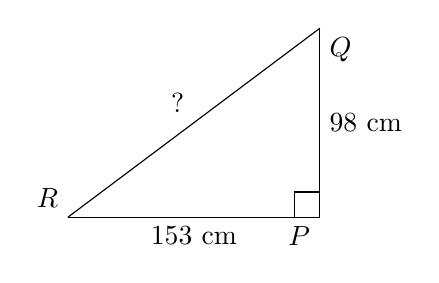
\begin{tikzpicture}[scale=0.4,rotate=90]
\coordinate (A) at (0,0); \coordinate (B) at (6,0); \coordinate (C) at
(0,8);

\draw (A) -- (B) node[midway,right] {98 cm}; \draw (A) -- (C)
node[midway,below] {153 cm}; \draw (B) -- (C) node[midway,above left]
{$?$};

\node[below left] at (A) {$P$}; \node[below right] at (B) {$Q$};
\node[above left] at (C) {$R$};

% Angle droit en A
\draw (0.8,0) -- (0.8,0.8) -- (0,0.8);
\end{tikzpicture}
\end{center}

\begin{enumerate}
\item \textbf{Égalité de Pythagore :} \\
\item \textbf{Remplacement :} \\ \\
\item \textbf{Calcul de la racine :} \\ \\
\item \textbf{Phrase réponse :} \\
\end{enumerate}
\end{exercice}


\end{document}

% Local Variables:
% gptel-model: deepseek-chat
% gptel--backend-name: "DeepSeek"
% gptel--bounds: ((response (345 1024) (1025 1093) (1116 1268) (1283 1285) (1301 1776) (1793 1830) (1831 1838) (1861 1937) (1967 1968) (1985 2463) (2480 2517) (2518 2528) (2551 2636) (2666 2667) (2692 3173) (3190 3227) (3228 3238) (3261 3345) (3376 3377)))
% End:
